\begin{mynotice} Элемент $1+kp$ также порождает $Ker$ $\pi$, если $k \not\equiv 0$ \linebreak $(mod p)$. \par

Отображение $\mathbb{Z}$ в $U({{\mathbb{Z}}_{p^{2}}})$, которое каждому числу b ставит в \linebreak соответствие $1-bp$, является гомоморфизмом, чье ядро --- $p \mathbb{Z}$, а \linebreak образ --- $Ker$ $\pi$. 
Это отображение индуцирует изоморфизм $\mathbb{Z}_{p}$ и \linebreak $Ker$ $\pi$. Если $x\in\mathbb{Z} - p\mathbb{Z}$, то разложение $U(\mathbb{Z}_{p^{2}})$, введенное в предло- \linebreak жении 35, позволяет записать $x$ = $x^{p}(x^{p-1})^{-1}$. По малой теореме \linebreak Ферма $x^{p-1}=1+a_{x}p$, а значит, $x\equiv x^{p}(1-a_{x}p) (mod \; p^{2})$, откуда \par  
\vspace{\baselineskip}
$$ x\equiv x^{p}(1-p)^{a_{x}} (mod \; p^2). $$ \par
\vspace{\baselineskip}
\noindent Это позволяет заключить, что в $U(\mathbb{Z}_{p^{2}})$ компонента $x$, принадле- \linebreak жащая $Ker$ $\pi$, есть степень $a_{x}$ образующей $1-p$ ядра $Ker$ $\pi$. \par
\vspace{\baselineskip}
\end{mynotice}
Предыдущее предложение позволяет полностью определить струк- \linebreak туру $U(\mathbb{Z}_{p^{r}})$ для нечетного простого p. Так как p - 1 и $p^{r-1}$ взаимно \linebreak просты и группа $U(\mathbb{Z}_{p^{2}})$ --- прямое произведение циклических групп \linebreak порядков $p-1$ и $p^{r-1}$, то она изоморфна $U(\mathbb{Z}_{p^{r-1}(p-1)})$ и циклична. \par
 
\vspace{\baselineskip}
\begin{thm}
\slshape{Пусть p --- нечетное простое число, а r --- строго положительное \linebreak целое число.} \par \slshape{(\textit{i}) Элемент $1-p$ имеет порядок $p^{r-1}$ в $U(\mathbb{Z}/p^{r})$.} \par 
\slshape{(\textit{ii}) Группа $U(\mathbb{Z}/p^{r}\mathbb{Z})$ изоморфна прямому произведению подгруппы \linebreak подрядка $p^{r-1}$, порожденной элементом $1-p$, и подруппы порядка $p-1$, \linebreak образованной q-ми степенями элементов  $U(\mathbb{Z}/p^{r}\mathbb{Z})$, где $q=p^{r-1}$. Вторая подруппа изоморфна  $U(\mathbb{Z}/p\mathbb{Z})$}. \par 
\slshape{(\textit{iii}) Группа $U(\mathbb{Z}/p^{r}\mathbb{Z})$ --- циклическая порядка $p^{r-1}(p-1).$}
\end{thm}
\noindent \textbf{Пример} \par
\upshape{В таблице 4 дана группа обратимых по модулю 125 элементов, разло- \linebreak женная согласно предыдущему изложению. В первом столбце находится \linebreak образ $\chi$, а в первой строке --- ядро $\pi$.} \par
Первый столбец состоит из 25-x степеней чисел по модулю 125 и \linebreak изоморфен $U(\mathbb{Z}_{5})$. При этом \textit{изоморфизме} элементы 57 и 68 соответ- \linebreak ствуют образующим группы $U({\mathbb{Z}_{5}})$. Кроме того, теперь легко опреде- \linebreak лить образ любого элемента из $U(\mathbb{Z}_{125})$ под действием $\chi$ : это элемент \linebreak первого столбца, который имеет тот же остаток по модулю 5. \par

\newpage
% новая страница 464 ---------------------------------

\begin{center}
    \begin{tabular}{| c | c | c | c | c | c | c | c | c | c | c | c | c | c }
    \hline
    \itshape{1} & \itshape{6} & \itshape{11} & \itshape{16} & \itshape{21} & \itshape{26} & \itshape{31} & \itshape{36} & \itshape{41} & \itshape{46} & \itshape{51} & \itshape{56} & \itshape{61} & ... \\ \hline
    \itshape{57} & \textbf{92} & \textbf{2} & \textbf{37} & \textbf{72} & 107 & \textbf{17} & \textbf{52} & \textbf{87} & \textbf{122} & 32 & \textbf{67} & \textbf{102} & ...
\\ \hline
    \itshape{68} & \textbf{33} & \textbf{123} & \textbf{88} & \textbf{53} & 18 & \textbf{108} & \textbf{73} & \textbf{38} & \textbf{3} & 93 & \textbf{58} & \textbf{23} & ...
\\ \hline
    \itshape{124} & 119 & 114 & 109 & 104 & 99 & 94 & 89 & 84 & 79 & 74 & 69 & 64 & ...
\\ \hline
    \end{tabular}
\end{center}

\begin{center}
    \begin{tabular}{| c | c  c | c | c | c | c | c | c | c | c | c | c | c }
    \hline
    \itshape{1} & ... & \itshape{66} & \itshape{71} & \itshape{76} & \itshape{81} & \itshape{86} & \itshape{91} & \itshape{96} & \itshape{101} & \itshape{106} & \itshape{111} & \itshape{116} & \itshape{121} \\ \hline
    \itshape{57} & ... & \textbf{12} & \textbf{47} & 82 & \textbf{117} & \textbf{27} & \textbf{62} & \textbf{97} & 7 & \textbf{42} & \textbf{77} & \textbf{112} & \textbf{22}
\\ \hline
    \itshape{68} & ... & \textbf{113} & \textbf{78} & 43 & \textbf{8} & \textbf{98} & \textbf{63} & \textbf{28} & 118 & \textbf{83} & \textbf{48} & \textbf{13} & \textbf{103}
\\ \hline
    \itshape{124} & ... & 59 & 54 & 49 & 44 & 39 & 34 & 29 & 24 & 19 & 14 & 9 & 4
\\ \hline
    \end{tabular}
\end{center}

\noindent \textbf{Таблица 4.} Разложение группы обратимых по модулю 125 элементов \par

\vspace{\baselineskip}

Первая строка представляет собой подгруппу $U(\mathbb{Z}_{125})$, изоморфную \linebreak $\mathbb{Z}_{25}$. Этот изоморфизм очень просто выражается в явном виде: он ото- \linebreak бражает элемент $x$ из $\mathbb{Z}_{25}$ в элемент $(1+5)^x$ из $U(\mathbb{Z}_{125})$, тем самым \linebreak преобразуя аддитивную структуру $\mathbb{Z}_{25}$ в мультипликативную струк- \linebreak туру подгруппы из $U(\mathbb{Z}_{125})$, образованной элементами, сравнимыми с \linebreak  1 по модулю 5. Эта подгруппа имеет 20 образующих (они выделены в \linebreak таблице курсивом). \par 
Группа $U(\mathbb{Z}_{125})$ есть прямое произведение первой строки и перво- \linebreak го столбца таблицы; ее образующие представляют собой произведения \linebreak образующих элементов из подгрупп, соответствующих первому столб- \linebreak цу и первой строке. Все образующие группы обратимых по модулю 125 \linebreak элементов выделены в таблице жирным шрифтом. Сколько же их? Не \linebreak трудно проверить, что их ровно $\varphi(\varphi(125)) = 40.$ \par
\vspace{\baselineskip}
Продолжим наше исследование. В случае $U(\mathbb{Z}_{{2}^{r}})$ мы выяснили, что \linebreak элемент 5 порождает \textit{подгруппу}  порядка $2^{r-2}$ при r > 2. Займемся те- \linebreak перь поиском примитивных корней в $U(\mathbb{Z}_{{p}^r}).$ \par

\begin{thm}
\slshape{Пусть p --- нечетное простое число. \par 
(\textit{i}) Пусть x обратимо по модулю p. Следующие утверждения экви- \linebreak валентны: \linebreak}
\indent \slshape{a) x --- примитивный корень по модулю $p^{r}$ для всякого r > 0, \linebreak \indent b)\; x --- примитивный корень по модулю $p^{r}$, \linebreak \indent c) x --- примитивный корень по модулю p и $x^{p-1} \not\equiv 1 \; ($mod$ \; p^{2}).$ } \par 
\slshape{(\textit{ii}) Пусть x --- примитивный корень по модулю p. Если $x\equiv y$ 
\linebreak $(mod \; p^{2})$ и $x \not\equiv y \; (mod \; p^{2})$, то один из элементов x или y является прими- \linebreak тивным корнем по модулю $p^{2}$. В частности, если x не является прими- } \linebreak \newpage

% новая страница 465 ----------------------------------

\noindent тивным корнем по модулю $p^{2}$, то $x+p$ и $x-p$ являются примитивными корнями по модулю $p^{2}$. 
\end{thm}
 \begin{myproof}
Импликации $a \rightarrow b \rightarrow c$ очевидны. Для доказательства $c \rightarrow a$ зап- \linebreak \indent ишем $x^{p-1} = 1 + kp$, где k не делится на p. Используя доказанные в \linebreak \indent предложении 31 (\textit{ii}) сравнения, получаем: \par 
$$x^{(p-1)p^{r-2}} \equiv 1 + kp^{r-1} (mod \; p^{r}),$$ \par 
\indent откуда следует, что порядок \textit{x} равен $(p-1)p^{r-1}$. \par 
\indent (\textit{ii}) Если $x \equiv y \; (mod \; p)$, то сформулированное в предложении 30 (\textit{ii}) \linebreak \indent соотношение приводит к $x^{p} \not\equiv y^{p} \; (mod \; p^{2})$. Остается лишь дока- \linebreak \indent зать, что $x^{p-1} \not\equiv y^{p-1} \; (mod \; p^{2})$, что равносильно $xy^{-1} \not\equiv 1 \linebreak \indent (mod \; p^{2})$. Если это не верно, то сравнение $xy^{-1} \equiv
1(mod \; p^{2})$ дава- \linebreak \indent ло бы $(xy^{-1})^{p} \not\equiv 1 \; (mod \; p^{2})$, что невозможно.
\end{myproof}
\begin{sled}
\slshape{Пусть x --- образующий группы $U(\mathbb{Z}/p^{r}\mathbb{Z})$, обратимый в $\mathbb{Z}/p\mathbb{Z}$, где \linebreak p --- нечетное простое число, $r \geqslant 1$}. Тогда остальные примитивные \linebreak корни по модулю $p^{r}$ являются степенями x, взаимно простыми с $\varphi(p^{r}) = \linebreak p(p - 1)$; их число равно $\varphi(\varphi(p^{r}))$, т.е. $p^{r - 2}(p - 1)\varphi(p - 1)$.
\end{sled}
\section{Почти периодические последовательности}
\noindent \upshape{Во многих областях математики бывает необходимо использовать так \linebreak называемые псевдослучайные последовательности чисел: в численных \linebreak методах это методы Монте-Карло, в статистике это генерирование \linebreak образцов для различных тестов, в некоторых алгоритмах требуется \linebreak выбрать \guillemotleft наугад\guillemotright \; один элемент из какого-то множества --- в этой главе \linebreak приведены конкретные примеры --- и такой случайный выбор может \linebreak значительно улучшить сложность алгоритма по отношению к выбору \linebreak детерминированному... Возникает множество вопросов относительно \linebreak так называемых \textit{генераторов случайных чисел}: насколько случайны по- \linebreak являющиеся числа? Что вообще такое последовательность случайных \linebreak чисел? Это довольно сложные вопросы.} \par 

Кнут[99] во введении к третьей граве \guillemotleft \textit{Случайные числа}\guillemotright \; своей кни- \linebreak ги, в качестве упражнения задает несколько вопросов, которые пока- \par

 \newpage


% новая страница 466 ----------------------------------

\noindent зывают, насколько наш выбор не случаен. Как, например, наугад \textit{вы- \linebreak брать} цифру от 0 до 9? Использовать телефонный справочник? Нет! \linebreak Цифры, которые там используются, неодинаково распределены. Попро- \linebreak сить кого-нибудь загадать цифру? Нет! В основном люди загадывают \linebreak вполне конкретные числа... \par 

Один из методов, используемых для образование чисел случайным \linebreak образом, состоит в применении последовательности, задаваемой срав- \linebreak нениями $x_{n+1} = ax_{n} + b \; mod \; m$. Конечно, эти последовательности на \linebreak некотором шаге становятся периодическими и нужно выбирать их так, \linebreak чтобы период был максимален. \par 

Известно, что десятичная запись рационального числа почти пе- \linebreak риодическая. Если открыть книгу, в которой изучаются непрерывные \linebreak дроби, то вскоре обнаружится, что запись непрерывной дроби действи- \linebreak тельного числа почти периодическая тогда и только тогда, когда это \linebreak число является квадратичным целым. Периодические явления встреча- \linebreak ются повсюду. В частности, всякий руррентный порцесс, происходя- \linebreak щий в конечном множестве, --- почти периодический (согласно прин- \linebreak ципу вложенных отрезков). В конце этого раздела мы увидим, что
в \linebreak некоторых случаях имеются эффективные алгоритмы для определения \linebreak периодов таких последовательностей, а в конце главы нами будет рас- \linebreak смотрен алгоритм факторизации, основанный на почти периодическом \linebreak явлении ($\rho$ -метод Полларда). \par

\subsection{Одношаговый генератор}

\noindent Случайные последовательности\footnote{Мы не будем доказывать никаких свойств этих последовательностей, касаю- \linebreak щихся их случайного ил детерминированного характера. Это выходит за рамки \linebreak данного учебника, требует серьезных статистических исследований и формального \linebreak определения того, что означает \guillemotleft наугад\guillemotright \;} легко получить при имитациях функ- \linebreak ций с одной или несколькими переменными (что влияет на длину по- \linebreak лучаемых последовательностей), выбранной таким образом, что пери- \linebreak одичность последовательностей неочевидна.

\begin{determ}
Последовательность $(x_{n})_{n}\geqslant 0$ (элементов какого-либо множества) на- \linebreak зывается периодической, если существует такое $k\geqslant 1$, что $x_{n+k} = x_{n}$ \linebreak для всех $n \in \mathbb{N}.$ Множество чисел k, удовлетворяющих этому определе- \linebreak нию, представляет собой подмножество из $\mathbb{N}^{*}$, замкнутое относитель- \linebreak но сложения и вычитания, и равное $\lambda \mathbb{N}^{*}$, где $\lambda$ --- наименьший элемент
 \newpage 
%новая страница 467 -----------------------------------
\noindent этого множества (как относительно отношения порядка $\leqslant$, так и по \linebreak делимости). \par 
Подпоследовательность $x_{0}, x_{1},..., x_{\lambda - 1}$ называется \textbf{периодом} по- \linebreak следовательности $(x_{n})_{n} \leqslant 0$, а число $\lambda$ --- \textbf{длиной периода}.
\end{determ}
\noindent\textbf{Пример} \par
\upshape{Последовательность десятичной записи числа 1/7 периодическая с \linebreak периодом длины 6, так как 1.7 = 0,\underline{142857}142857...}. Последователь- \linebreak ность $x_{n+1} = 4x_{n}, x_{0} = 5$ имеет период длины 3. Этот период \linebreak (5, 20, 17).


\begin{determ}
\slshape{Последовательность $(x_{n})_{n} \geqslant 0$} называется \textbf{почти периодической} \linebreak или \textbf{периодической некоторого ранга}, если существует такое \linebreak $m \geqslant 0$, что последовательность $(x_{n})_{n \leqslant m}$ периодическая. Обозначим че- \linebreak рез $\mu$ наименьшее из целых чисел m, удовлетворяющих этому свойству. \linebreak $\mu$ называется \textbf{индексом вхождения в период}. Назовем \textbf{периодом \linebreak последовательности} $(x_{n})_{n} \geqslant 0$ период последовательности $(x_{n})_{n \geqslant \mu}$. \linebreak Отметим, что множество \par 
{$${k \in \mathbb{N}|\exists m, x_{n+k} = x_{n}, \forall n \geqslant m},$$} \linebreak
как и в предыдущем определении, есть множество кратных длине пе- \linebreak риода.
\end{determ}
\textbf{Примеры} \par
\upshape{Последовательность $x_{n+1} = 2x_{n}+1 mod \; 48, x_{0} = 0,$ является перио- \linebreak дической ранга 4 и имеет период длины 2:} \par 
$$\;\;\;\;\;\;\;\;\;\;\;\;\;\;\;\;\;\;\;\;\;\;\;\;\;\;\;\;\;\downarrow \leftharpoonup \uparrow$$
$$0 \to 1 \to 3 \to 7 \to 15 \to 31$$ \par 
Для числа $\frac{99}{700} = 0,14\underline{142857}142857...$ последовательность десятичной \linebreak записи почти периодическая, а последовательность десятичной запи- \linebreak си $\sqrt{2} = 1,4142135623730950488016887242096980785697...$ не являет- \linebreak ся почти периодической. \par 
В данном разделе \textbf{генератором} множества F называется алго-\linebreak ритм, который выдает последовательность $(x_{n})_{n}\geqslant 0$ элементов F. На- \linebreak пример, \par 
$$x_{n+1} = 3141592521 x_{n} + 2718281829 (mod \; 10^{10}),$$
$$x_{n} = (x_{n-24}+x_{n-55})(mod \; 2^{64}),$$
$$x_{n+1} = (4x_{n}^{2} + 5x_{n})(mod \; 2^{32}).$$ \par \newpage 

%страница 468 ----------------------------------------

\noindent В дальнейшем будем считать, что $F$ \textbf{конечно}, и рассматривать только \linebreak \textbf{одношаговые} генераторы, т.е. имеющие вид $x_{n+1} = f(x_{n})$, где $f$ --- \linebreak отображение $F$ в себя. \par 
\begin{predl}
Пусть $(F,f,x_{0})$ --- генератор (множество $F$ конечно). Тогда после- \linebreak довательность $(x_{n})_{n \geqslant 0}$, определяемая по правилу $x_{n+1} = f(x_{n})$, почти \linebreak периодическая. Если $\mu$ --- индекс вхождения в период, а $\lambda$ --- длина \linebreak периода, то для различных индексов \textit{i} и \textit{j} \par

$$x_{i}=x_{j} \Longleftrightarrow \textit{i},\textit{j} \geqslant \mu и \textit{i}\equiv\textit{j} (mod \; \lambda).$$ \par 
\noindent В частности, все $x_{\textit{i}}$ при $0 \leqslant\textit{i} \leq \mu + \lambda$ попарно различны и, следователь- \linebreak но, $\mu + \lambda \leqslant|F| и \mu \leqslant|F| - 1)$. \par 
\end{predl}
\begin{myproof}
Поскольку F конечно, существую h < k такие, что $x_{h} = x_{k}$ (прин- \linebreak \indent цип ящиков). Применяя $f^{r}$, получим $x_{h+r} = x_{k+r}$, а значит, k - h --- \linebreak \indent период подпоследовательности $(x_{i})_{i}\geqslant h$. Предположим, что $x_{i} = x_{j}$ \linebreak \indent  для $j > i$. Последовательность $(x_{l})_{l \geqslant i}$ периодична, а потому $i \geqslant \mu$ и, \linebreak \indent следовательно, $j - i \equiv 0 (mod \; \lambda)$. Обратное очевидно, так же как и \linebreak \indent конец предложения. \par 
\end{myproof}
\begin{figure}[h]
\center{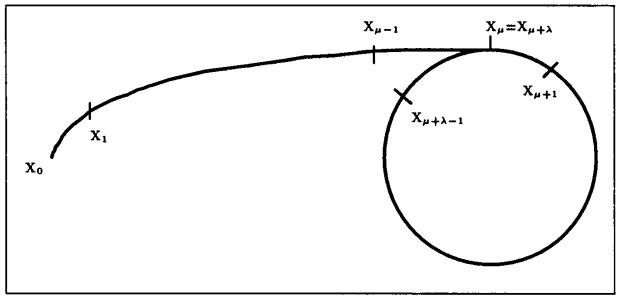
\includegraphics[width=0.8\linewidth]{image3}}
\end{figure}

Почти периодическая последовательность, получаемая при одноша- \linebreak говом генерировании, схематически может быть представлена фигурой \linebreak $\rho$(рис. 1): все элементы на $\rho$ различны, хвост --- это множество членов \linebreak \newpage

%новая страница 469-----------------

\noindent последовательности, которые не входят в период, а завиток предста- \linebreak вляет собой пеирод. Число $\mu$ является длиной хвоста, а $\lambda$ --- длиной \linebreak завитка. \par 
\vspace{\baselineskip}
\noindent \textbf{Пример: представление рационального числа в виде \linebreak десятичной дроби}
\upshape{Пусть $u$ и $v$ --- два целых числа с $v > 0$ и $q_{0} + (0 \cdot q_{1}q_{2}...)_{10}$ --- де- \linebreak сятичная запись числа $u / v$ с $q_{0} \in \mathbb{N}$. Можно определить последователь- \linebreak ность $({r_{i}})_{i \geqslant 0}$ по правилу: $r_{0} = u, r_{i+1} = 10r_{i} mod v$. Тогда $q_{i+1} = [\frac{10r_{i}}{v}]$ \linebreak (и $q_{0} = [u / v]$). Последовательность $r_{i}$ порождается с функцией $f:[0, v[ \to$ \linebreak $[0, v[$, которая каждому x ставит в соответствие $10 x mod v$. Такая по- \linebreak следовательность почти периодическая, а потому почти периодической \linebreak является и последовательность $q_{i}$ десятичных цифр в записи $u / v$.} \par 
\begin{mynotice}Отметим, что индекс вхождения в период и длина \linebreak \indent периода зависят от первого члена $x_{0}$. Например, для последова- \linebreak \indent тельности $x_{n+1} = 2x_{n} + 1 (mod 48)$ имеем: \linebreak
 
$\;\;\;\;\; \downarrow \leftharpoonup \uparrow$ \linebreak
\indent $(i)$ при $x_{0} = 0: 0 \to 1 \to 3 \to 7 \to 15 \to 31$, а значит, $\mu = 4, \linebreak \lambda = 2,$ \par 

$(ii)$ при $x_{0} = 11: 11 \to 13 \to 47 \to$ и уже $\mu = 2, \lambda = 1.$ \par 

Хотя одношаговый генератор не может порожать последо- \linebreak \indent вательности, период которых больше порядка F, очевидно, су- \linebreak \indent ществуют почти периодические последовательности произвольно \linebreak \indent большого периода. Например, для F = {0,1} последовательность \linebreak \indent $(x_{n})_{n \geqslant 0}$ такая, что $x_{n} = 0$ при $n \not\equiv 0 (mod \lambda)$ и $x_{n} = 1$ при \linebreak \indent $n \equiv 0 (mod \lambda)$ имеет период длины $\lambda$. Так как для $\lambda = 5$ получаем \linebreak \indent 0000100001.... \par 
Предыдущий пример тривиален, а потому приведем еще один \linebreak пример: \par 
\noindent $1 \, \to \, 1 \, \to \, 0 \, \to \, 1 \, \to \, 0 \, \to \, 1 \, \to \, 0 \, \to \, 0 \, \to \, 0 \, \to \, 0 \, \to \, 0 \, \to \, 1 \, \to \, 0 \, \to \, 0 \, \to \, 1$ \linebreak
$\uparrow \;\;\;\;\;\;\;\;\;\;\;\;\;\;\;\;\;\;\;\;\;\;\;\;\;\;\;\;\;\;\;\;\;\;\;\;\;\;\;\;\;\;\;\;\;\;\;\;\;\;\;\;\;\;\;\;\;\;\;\;\;\;\;\;\;\;\;\;\;\;\;\;\;\;\;\;\;\;\;\;\;\;\;\;\;\;\;\;\;\;\;\;\;\;\;\;\;\;\;\;\;\;\;\;\;\;\;\;\;\;\;\;\;\;\;\;\;\;\;\;\;\;\;\;\;\;\downarrow$ \linebreak
$ 1 \;\;\;\;\;\;\;\;\;\;\;\;\;\;\;\;\;\;\;\;\;\;\;\;\;\;\;\;\;\;\;\;\;\;\;\;\;\;\;\;\;\;\;\;\;\;\;\;\;\;\;\;\;\;\;\;\;\;\;\;\;\;\;\;\;\;\;\;\;\;\;\;\;\;\;\;\;\;\;\;\;\;\;\;\;\;\;\;\;\;\;\;\;\;\;\;\;\;\;\;\;\;\;\;\;\;\;\;\;\;\;\;\;\;\;\;\;\;\;\;\;\;\;\;\;\; 0$ \linebreak
$\uparrow \;\;\;\;\;\;\;\;\;\;\;\;\;\;\;\;\;\;\;\;\;\;\;\;\;\;\;\;\;\;\;\;\;\;\;\;\;\;\;\;\;\;\;\;\;\;\;\;\;\;\;\;\;\;\;\;\;\;\;\;\;\;\;\;\;\;\;\;\;\;\;\;\;\;\;\;\;\;\;\;\;\;\;\;\;\;\;\;\;\;\;\;\;\;\;\;\;\;\;\;\;\;\;\;\;\;\;\;\;\;\;\;\;\;\;\;\;\;\;\;\;\;\;\;\;\;\downarrow$ \linebreak
\noindent $0 \, \to \, 1 \, \to \, 1 \, \to \, 0 \, \to \, 0 \, \to \, 0 \, \to \, 1 \, \to \, 1 \, \to \, 1 \, \to \, 1 \, \to \, 1 \, \to \, 0 \, \to \, 0 \, \to \, 1 \, \to \, 1$ \linebreak

\indent В данном случае используется множество {0,1} и если приc- \linebreak мотреться повнимательнее, то видно, что все 5-ти битовые цепи \linebreak возникают в данной диаграмме ровно по одному разу. Этот цикл \linebreak длины 32, а значит, генерируется за 5 шагов. Этому циклу отве- \linebreak чает многочлен степени 5, неприводимый над $\mathbb{Z}_{2}$, $P = X^{5} + X^{5} + 1$.
\end{mynotice}
\newpage

%новая страница 470-----------------------------------------------

\begin{determ} 
\textit{Одношаговый генератор $(F,f,x_{0})$ называется генератором \textbf{максимального периода}, если длина его периода равна |F|}.
\end{determ}
\begin{predl}
\slshape{Для одношагового генератора (F,f) эквивалентны следующие усло- \linebreak вия:} \par 
\upshape{a)$(F,f,x_{0})$ максимального периода для $x_{0} \in F$. \par 
\indent b)Отображение f --- циклическая перестановка F. \par
\indent c)$(F,f,x)$ максимального периода для всех $x \in F$. \par
\indent d)Для любых $x,y \in F$ существует $r \in \mathbb{N}$ такое, что $f^{r}(x) = y.$ \par}
\indent Из двух генераторов $(F,f,x_{0})$ и $(G,g,y_{0})$ можно получить третий, \linebreak рассматривая их декартово произведение $(F \times G, f \times g, (x_{0}, y_{0})).$
\end{predl}
\begin{predl}
 \slshape{Декартово произведение двух генераторов имеет период длины, \linebreak равной НОК длин периодов компонент, а индекс вхождения, равный \linebreak наибольшему из индексов компонент.}
\end{predl}
\begin{myproof}
 Для последовательности $(u_{n})_{n \geqslant 0}$ обозначим: \par 
 $$I_{u} = {s \equiv \mathbb{N}|\exists k_{0}, u_{k+s} = u_{k}, \forall k \geqslant k_{0}}.$$ \par 
 Тогда для последовательностей $(x_{n})_{n \geqslant 0}, (y_{n})_{n \geqslant 0}, (z_{n})_{n \geqslant 0},$ порожда- \linebreak \indent емых соответственно функциями $f, g$, и $f \times g$, имеем $I_{x} \bigcap I_{y} = I_{z}$, \linebreak \indent откуда легко получить утверждение, касающееся длины периода. \linebreak \indent Последовательность $(z_{i})_{i \geqslant q}$ периодична тогда и только тогда, когда \linebreak \indent такими же являются последовательности $(x_{i})_{i \geqslant q}$ и $(y_{i})_{i \geqslant q}$, до- \linebreak \indent казывает утверждение относительно индекса вхождения в период. \par 
\end{myproof}
\subsection{Генерирование при помощи линейных сравнений}

\noindent В данное пункте рассматриваются генераторы вида \par 
$$x_{n+1} = ax_{n} + b mod \; m;$$ \par
\noindent назовем их линейными генераторами сравнений. Такие генераторы ха- \linebreak рактеризуются модулем m, \textit{аффинным} преобразованием $x \to ax + b$ кольца $\mathbb{Z}_{m}$ (назовем a мультипликатором, а b приращением) и, нако- \linebreak нец, первым членом $x_{0} \in \mathbb{Z}_{m}$. \par \newpage 

%новая страница 471----------------------

\textbf{Несколько примеров} \begin{itemize}
\item $x_{n+1} = 4x_{n}+1 \; mod \; 9, x_{0} = 0$ дает 
$$0 \to 1 \to 5 \to 3 \to 4 \to 8 \to 6 \to 7 \to 2$$
\item $x_{n+1} = 2x_{n} + 1 \; mod \; 48, x_{0} = 0$ дает $0 \to 1 \to 3 \to 7 \to 15 \to 31$
\item $x_{n+1} = 3x_{n} + 1 \; mod \; 20, x_{0} = 0$ дает $0 \to 1 \to 4 \to 13$
\item $x_{n+1} = 2x_{n} + 1 \; mod \; 5, x_{0} = 0$ дает цикл $0 \to 1 \to 3 \to 2$, а при \linebreak $x_{0} = 4$ цикл длины 1: (4).
\end{itemize}
Дадим теперь необходимые и достаточные условия того, что генера- \linebreak  тор сравнений имеет максимальный период. Более детальное изучение \linebreak читатель найдет в упражнениях 37-40. \par 
\begin{predl} (китайская теорема об остатках). \par
\indent\slshape{Пусть $m = m_{1}m_{2}$, где  $m_{1}$ и $m_{2}$} --- два взаимно простых числа. Любой \linebreak генератор сравнений по модулю $m$: \par 

\begin{equation*}
(G) 
 \begin{cases}
   &\text{$z_{n+1} = (az_{n} + b) \; mod \; m$}\\
   &\text{$z_{0} = c \; mod \; m$}
 \end{cases}
\end{equation*}

\noindent есть декартово произведение генераторов по модулям $m_{1}$ и $m_{2}$: \linebreak
 
 \begin{equation*}
(G) 
 \begin{cases}
   &\text{$x_{n+1} = (ax_{n} + b) \; mod \; m_{1}$}\\
   &\text{$x_{0} = c \; mod \; m_{1}$}
 \end{cases}
\end{equation*}
 
 
\noindent В частности, длина периода (G) равна НОК длин периодов ($G_{1}$) и ($G_{2}$), \linebreak а индекс вхождения в период (G) равен наибольшему из индексов вхо- \linebreak ждения ($G_{1}$) и ($G_{2}$). \par
\end{predl} 
\begin{myproof}
Рассмотрим преобразования $f_{1}, f_{2}, f_{3}$, определенные по правилам \linebreak \indent $f_{1}(x) = ax + b \; mod \; m_{2}, f(z) = az + b \; mod \; m.$ \linebreak \indent Тогда коммутативна диаграмма \par 

$$\mathbb{Z_{m}} \to \mathbb{Z_{m}} \linebreak \indent
 \downarrow \;\;\;\;\;\;\;\;\;\;\;\;\;\;\;\; \uparrow \linebreak \indent
 \mathbb{Z_{m_{1}}} \times \mathbb{Z_{m_{2}}} \to \mathbb{Z_{m_{1}}} \times \mathbb{Z_{m_{2}}}$$ \par 
 в которой вертикальные отображения --- это китайский изомор- \linebreak \indent физм $\bar{z_{m_{1}}} \to (\bar{z_{m_{1}}}, \bar{z_{m_{2}}})$ и, следовательно, f и $f_{1} \times f_{2}$ связаны между \linebreak \indent собой. \end{myproof}
 \newpage
 
 % новая страница 472
 
После этого общего представления генераторов сравнений, займем-  \linebreak ся теми, которые имеют максимальный период. \linebreak 
\indent Предположим, что генератор $x_{n+1} = f(x_{n}) = ax_{n} + b \; mod \; m$ имеет \linebreak максимальный период (т.е. период длины m). Тогда для всякого дели- \linebreak теля $p \geqslant 2$ числа m генератор $x \mapsto ax + b \; mod \; p$ также имеет период \linebreak длины p. Действительно, если f --- цикл на множестве A, а $\pi$ ---сюръ- \linebreak екция A на множество B, то преобразование g множества B такое, что \linebreak $\pi \circ f = g \circ \pi$, также является циклом. Поэтому, если последовательность \linebreak имеет максимальную длину, то уравнение $x = ax + b \; mod \; p$ не имеет ре- \linebreak шений для любого делителя p числа m. В частности, если p --- простое, \linebreak то: \par
$$a - 1 \equiv 0 \; (mod \; p) и\; b \not\equiv 0 \; (mod \; p).$$ \par 
\noindent Кроме того, если 4 делит m, то $a \equiv 1 (mod \; 4)$. Действительно, $a \equiv 1 \linebreak (mod \; 2)$  и условие$ a \equiv -1 (mod \; 4)$ невозможно, так как тогда \linebreak $x_{n+1} = -x_{n} + b \; mod \; 4$. Эти условия являются и \linebreak достаточными, как это следует их следующей теоремы. \par 

\begin{thm}
\textit{Генератор сравнений $x_{n+1} = f(x_{n}) = ax_{n} + b \; mod \; m$ имеет максимальный период тогда и только тогда, когда выполняются следующие \linebreak три условия:} \par 
a) b обратимо по модулю m, \linebreak
\indent b) $a \equiv 1 (mod \; p)$ для любого простого p, делящего m, \linebreak
\indent c) если 4 делит m, то $a \equiv 1 (mod 4).$ \par
\end{thm}
\begin{lemma}
Пусть f(x) = ax + b рассматривается как отображение $Z_{m}$ в себя. \linebreak Тогда q-я степень f это афинное преобразование $x \to a^{q}x + bS_{q}(a)$, \linebreak $S_{q}(X)$ --- многослен из раздела 3.4.1. В частности, если b обратимо по \linebreak модулю m, то \par
$$f^{q}(0) = 0 \Leftrightarrow S_{q}(a) = 0 \Leftrightarrow f^{q} = Id_{\mathbb{Z_{m}}}.$$ \par
\end{lemma}
\upshape{Чтобы доказать эту лемму, достаточно заметить, что $bS_{q}(a) = 0$ \linebreak эквивалентно $S_{q}(a) = 0$, так как b обратимо по модулю m, и что \linebreak $S_{q}(a) = 0$ влечет $a^{q} = 1$, ибо $a^{q} - 1 = (a - 1)S_{q}(a).$
\begin{lemma}
\slshape{Пусть p --- простое, $r \geqslant 1 (с r = 1$ при $p = 2), a \equiv 1 (mod \; p)$ и $b \not\equiv 0 \linebreak (mod \; p).$ Тогда $x \mapsto f(x) = ax + b$ --- циклическая перестановка $\mathbb{Z_{p^{r}}}$, а \linebreak значит, генератор максимального периода.}  \par \newpage 
\end{lemma}
%новая страница 473--------------------------------------------
\begin{myproof}
Отображение f это перестановка $Z_{p^{r}}$, так как a обратимо по моду- \linebreak \indent лю $p^{r}$. Кроме того, лемма тривиальна, если $p = 2$(так как r = 1). \linebreak \indent Предположим, что $p \ne 2$, и рассмотрим ограничение f на орбиту 0, равную \linebreak \indent ${f^{q}(0), q \equiv \mathbb{N}}$. Достаточно доказать, что наименьшее q та- \linebreak \indent кое, что $f^{q}(0) = 0$, равно $p^{r}$. Так как $a \equiv 1 (mod \; p)$, то $S_{p^{r}}(a) \equiv 0 \linebreak \indent (mod \; p^{r})$ согласно предложению 31, имеем $S_{p^{r}}(a) \not\equiv p^{l} (mod \; p^{l + 1})$ и, следова- \linebreak \indent тельно, $S_{p^{l}}(a) \not\equiv 0 (mod \; p^{r})$. Теперь осталось применить лемму 48.
\end{myproof}
\begin{lemma}
\slshape{Пусть $r \geqslant 2$, а $a \equiv 1 (mod \; 4)$ и $b \not\equiv 0 (mod \; 2)$. Тогда $x \mapsto f(x) = \linebreak ax + b$ --- циклическая перестановска $\mathbb{Z_{2^{r}}}$, а значит, генератор макси- \linebreak мального периода.}
\end{lemma}
\begin{myproof}
 \indent\upshape{Доказательство аналогично доказательству предыдущей леммы и \linebreak \indent использует главным образов то, что $a \equiv 1 (mod \; 2^{2})$. Согласно \linebreak \indent предложению 32 имеем $S_{p^{r}}(a) \equiv 0 (mod \; 2^{r})$, а кроме того, при \linebreak \indent $l < r, S_{2^{l}}(a) \equiv 2^{l} (mod \; 2^{l+1})$, по предложению 32, откуда $S_{2^{l}}(a) \not\equiv 0 \linebreak \indent (mod \; 2^{r})$. Затем применим лемму 48.} \par 
\end{myproof}
Теперь можно доказать теорему 47. Необходимость доказана перед \linebreak формулировкой теоремы, а достаточность следует из китайской тео- \linebreak ремы об остатках и двух предыдущих лемм. \par 
\textbf{Пример} \par
Пусть $m = 10^{6} - 1 = 3^{3} \times 7 \times 11 \times 13 \times 37$. Чтобы получить генератор \linebreak $x_{n+1} = ax_{n} + b \; mod \; m$  максимального периода, нужно выбрать (согласно \linebreak теореме 47): \par 
$$a \equiv 1 (mod 3 \times 7 \times 11 \times 13 \times 37) и b \not\equiv 0 (mod \; p)$$
$$для p \in \{3, 7, 11, 13, 37\}.$$
\noindent Это дает 9 решений для $a$ вида $1 + 111111 \times с 0 \geqslant k \geqslant 8.$
\subsection{Нахождение периода методом Брента}
\noindent Пусть f --- конечно множество, $x_{0} \in F$ и $f: F \to F$ отображение, которому соответствует последовательность $x_{n+1} = f(x_{n})$, начинаю- \linebreak щаяся с $x_{0}$. Цель алгорима Брента --- сосчитать длину периода после- \linebreak довательности $((x_{n})_{n \geqslant 0}$, используя при этом как можно меньше памяти \linebreak

% новая страница 474 ------------------------------------------

\noindent(достаточно 3 переменных!). Сложность алгоритма имеет порядок ква- \linebreak дратного корня из F.} \par 

\slshape{\textbf{Принцип метода}} \par
\upshape{Метод Брента состоит в проверке равенства $x_{h} = x_{k}$ для пар ин- \linebreak дексов (h,k), принимающих следующие значение:} \par
\begin{figure}[h]
\center{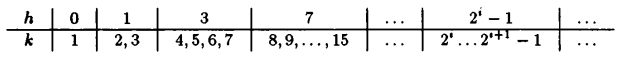
\includegraphics[width=1\linewidth]{image4}}
\end{figure}% таблица
Отметив, что для $h = 2^{i} - 1$ интервал соответствующих значений k равен $[h + 1, 2h + 1]$. Для того, чтобы теперь $x_{h} = x_{k}$, необходимо
\begin{wrapfigure}{i}{0.5\textwidth}
\begin{lstlisting}[mathescape=true]
$j \leftarrow 1; x \leftarrow x_0;j - 1 = h$
$\text{loop}$
 $x' \leftarrow{x};$
 $j \text{ - степень } 2,\text{ } x' = x = x_{j-1}$
 $\text{for }\lambda \text{ in } 1..j \text{ loop } j - 1 + \lambda = k$
  $x\leftarrow f(x); x = x_{j-1+\lambda}$
  $x'={x'} \text{ then}$
  $\text{return } \lambda;\text{ длина периода}$
  $\text{end if};$
 $\text{end loop};$
 $j\leftarrow 2j;$
$\text{end loop};$
\end{lstlisting}
Алгоритм 4. Вычисление\\
периода по методу Брента
\end{wrapfigure}
 и достаточно, чтобы $h \geqslant \mu$ (индекс вхождения в период) и k - h было  кратно $\lambda$ (длина периода) --- условия, которые выполняются при достаточно большом h (так как интервал для k удваивается на каждом этапе). Пусть h --- какой-либо индекс, для которого существует  $k \in [h + q, 2h + 1]$ с $x_{h} = x_{k}$. Если k --- первый индекс интервала $[h + q, 2h + 1]$, для которого $x_{h} = x_{k}$, то k - h равно длине периода $\lambda$. Наконец, если $\mu$ --- наименьший индекс, такой, что $x_{\mu} = x_{\mu + \lambda}$, то $\mu$ --- индекс вхождения в пеирод. Это приводит к алгоритму, представленному слева. В этом алгоритме переменная j принимает значения h + 1, т.е. степени 2. Хотя алгоритм 4 находит только длину периода, дальнейшее применение метода Брента позволяет определить все 4 параметра $(h, k, \mu, \lambda)$, описанных выше (причем $k - h = \lambda$): сложность измеряется при помощи параметра k, который равен числу итераций $x \leftarrow f(x)$ и обозначается $k_{f,x_{0}}$. \par 

\noindent\slshape{\textbf{Пример}} \par 
\upshape{Применяя метод Брента к десятичной записи числа $\frac{1}{7^{2}}$, получаем:} \par 
$$\frac{1}{49} = 0.\underline{020408163265306122448979591836734693877551}020408163...$$ \par 
\indent Длина периода равна 42 и в этом нет ничего удивительного, так как при \linebreak получении цифр десятичной записи используется функция \linebreak\newpage 

% новая страница 475--------------------------------------------

\noindent$x \mapsto 10x \; mod]; 7^{2}$ и длина периода равна порядку элемента 10 в суль- \linebreak типликативной группе $U(\mathbb{Z^{7_{2}}})$. Но 10 --- порождающий элемент \linebreak группы $U(\mathbb{Z^{7_{2}}})$ и $10^{7-1} \not\equiv 1 (mod \; 7^{2})$, а значит, 10 --- порождающий элемент \linebreak группы $u(\mathbb{Z^{7_{2}}})$ и его порядок $\phi(7^{2}) = 42$. \par 

\noindent\slshape{\textbf{Сложность метода Брента}} \par 
\upshape{Рассмотрим теперь следующую проблему: если f --- функция, дей- \linebreak ствующая из F в F, и начальный член $x_{0} \in F$ "выбран наугад", то \linebreak каков порядок величин $\lambda$ (длина периода), $\mu$ (индекс вхождения алгоритма в пе- \linebreak риод) и индекса $k = k_{f,x_{0}}$, полученного после применения алгоритма \linebreak Брента? Основной результат данного раздела состоит в том, что эти \linebreak величины имеют порядок $\sqrt{m}$, где m --- число элементов в F. Основ- \linebreak ные идеи доказательства заимствованы из книги Кнута "The Art Of \linebreak Computer Programming", успржнения к разделам 3.1 и 4.5.4. Читатель \linebreak может также обратиться к [104], [155] и [67].} \par 
Заметим сначала, что если $\mu$  --- индек с вхождения, то выполняется \linebreak равенство (в котором сложное выражение $2^{[log_{2}n])}$ --- это наименьшая \linebreak степень 2б большая или равная n): \par 
$$k_{f,x_{0}} = 2^{[log_{2}max(\mu+1,\lambda)]} + \lambda - 1$$ \par 
\noindent Действительно, $h = k_{f,x_{0}} - \lambda$ --- это наименьшее целое число, такое, что: \par 

$$h + 1 степень 2 и h \geqslant \mu, (2h + 1) - h \geqslant \lambda.$$ \par 
\noindent Значит h, удовлетворяющее этим условиям, равно $2^{[log_{2}max(\mu + 1,\lambda)]} - 1$, \linebreak откуда и следует равенство для $k_{f,x_{0}}$. Заметим, что $k_{f,x_{0}}$ зависит только \linebreak от $\lambda$ или $\mu$, а потому обозначим его через $k_{\mu, \lambda}$. \par 
Зафиксируем конечное множество F мощности m и рассмотрим ве- \linebreak роятностное пространнство, состоящее из возможных пар $(f, x_{0})$, где \linebreak $f: F \to F$ --- некоторая функция, а $x_{0} \in F$. \par 

\begin{lemma}
Пусть F --- конечное множество мощности m и $\lambda$, $\mu$ удовлетворяют \linebreak неравенствам $1 \geqslant \lambda \geqslant m, 0 \geqslant \mu и \mu + \lambda \geqslant m$. Вероятность того, \linebreak что последовательность $x_{n+1} = f(x_{n})$(f --- функция из F в F, $x_{0} \in F$) \linebreak имеет   период длины $\lambda$ и индекс вхождения $\mu$, равна \par 

$$P(\mu, \lambda)=\frac{1}{m} \Pi_{1\geqslant k<\mu+\lambda} (1 - \frac{k}{m}).$$ \par 
\noindent Функция $P(\mu,\lambda)$ зависит только от $\mu + \lambda$ (и m, очевидно). \end{lemma}
\newpage 
%новая страница 476--------------------------------------------

\begin{myproof}
Имеется $m^{m+1}$ возможностей выбора функции f из F в F (число \linebreak которых $m^m$) и первого члена $x_{0}$. Благоприятным исходом, кото- \linebreak \indent рому соответствует пара $(f, x_{0})$, является последовательность из \linebreak \indent $\mu + \lambda$ различных элементов $E = (x_{0}, x_{1},..., x_{\mu + \lambda -1})$(на которой f \linebreak \indent зацикливается) и произвольная функция из $F - E$ в F (сужение f \linebreak \indent на $F - E$). Число благоприятных исходов равно \par 

$$m \times (m - 1) \times ... \times (m -(\mu + \lambda - 1)) \times m^{m - (\mu + \lambda)}.$$ \par 
Значит, отношение числа благоприятных исходов к общему числу возможностей равно: \par 

$$\frac{m \times (m - 1) \times ... \times (m - (\mu + \lambda - 1))}{m^{\mu + \lambda + 1}} =$$ $$= \frac{1}{m} \times (1 \ \frac{1}{m})\times ... \times (1 - \frac{\mu + \lambda - 1}{m}).$$ \par 
\end{myproof}
\begin{determ}
\slshape{Определим функцию $Q : \mathbb{N^{*}} \to \mathbb{R^{+}}$ следующим образом \par}

$$ Q(m) = 1 + \frac{m - 1}{m} + \frac{m - 1}{m}\frac{m - 2}{m} +...+\frac{m - 1}{m}\frac{m - 1}{m}...\frac{1}{m}$$ \linebreak
$$= \sum_{1 \geqslant q \geqslant m} \Pi_{1 \geqslant k \geqslant q}(1 - \frac{k}{m}) = \sum_{1 \geqslant q \geqslant m} \frac{m!}{(m - q)!m^{q}}.$$ \par 
\noindent Она связана с $P(\mu, \lambda)$ равенством $\sum_{0 \geqslant \mu \geqslant m}P(\mu,1) = Q(m)/m.$ \par 
\end{determ}
\begin{predl}
\slshape{Кнутом в книге The Art Of Computer Programming, раздел 1.2.11.3, была получена асимптотическая формула для функции Q:} \linebreak 

$$Q(n) = \sqrt{\frac{\pi n}{2}} - \frac{1}{3} + \frac{1}{12}\sqrt{\frac{\pi}{2n}} - \frac{4}{135n} + \frac{1}{288}\sqrt{\frac{\pi}{2n^{3}}} + O(n^{-2}).$$ \par 

\upshape{Функция Q используется при изучении сложности алгоритма Брен- \linebreak та.} \linebreak
\end{predl}
\begin{lemma}
\slshape{Если индексы $\lambda$ и $\mu$ связаны соотношениями $1 \geqslant  \lambda \geqslant m, 0 \geqslant \mu < m$ \linebreak \newpage 

% новая страница 477-------------------------------------------

и $\mu + \lambda \leqslant m$, то выполняются равенства:} \par
 
$$\sum_{\mu,\lambda} P(\mu,\lambda) = \frac{1}{m} \sum_{1 \leqslant q < m} q \Pi_{1 \leqslant k < q} (1 - \frac{k}{m}) = 1,$$ \par 

$$\sum_{\mu,\lambda} (\mu + \lambda) P(\mu,\lambda) = \frac{1}{m} \sum_{1 \leqslant q < m} q^{2} \Pi_{1 \leqslant k < q} (1 - \frac{k}{m}) = Q(m),$$ \par 

$$\sum_{\mu,\lambda} \lambda P(\mu,\lambda) = \frac{1}{m} \sum_{1 \leqslant q < m} \frac{q(q+1)}{2} \Pi_{1 \leqslant k < q} (1 - \frac{k}{m}) = \frac{Q(m)+1}{2},$$ \par 

$$\sum_{\mu,\lambda} \mu P(\mu,\lambda) = \frac{1}{m} \sum_{1 \leqslant q < m} \frac{q(q-1)}{2} \Pi_{1 \leqslant k < q} (1 - \frac{k}{m}) = \frac{Q(m)-1}{2}.$$ \par

\noindent Эти равенства представляют собой математические ожидания соответ- \linebreak ственно 1, $\mu + \lambda, \lambda и \mu$. \par
\end{lemma}
\begin{myproof}
\indent Заметим, что \linebreak 
$$\sum_{\mu,\lambda} g(\mu, \lambda) P(\mu, \lambda) = \sum_{1 \leqslant q < m} \sum_{\mu + \lambda = q} g(\mu, \lambda) =$$ \par 
$$\frac{q}{m} \sum_{1 \leqslant q < m} \sum_{1 \leqslant \lambda < q} g(q - \lambda,\lambda) \Pi_{1 \leqslant k < q} (1 - \frac{k}{m}),$$ \par 

что позволяет перейти от выражений с $(\mu, \lambda)$ к выражениям с q. \linebreak \indent Функция $P(\mu, \lambda)$ была определена как вероятность и, следователь- \linebreak \indent но, $\sum_{\mu,\lambda} P(\mu,\lambda) = 1$ (первая формула леммы). \linebreak \indent
Для бесконечной последовательности $a = (a_{0}, a_{1}, a_{2},...)$ 
 определим \linebreak \indent f(a): \par 
 $$f(a) = f(a_{0}, a_{1}, a_{2},...) = \sum_{n \geqslant 0} a_{n} \Pi_{1 \leqslant k \leqslant n} (1 - \frac{k}{m}) = $$ \par
 
 $$= a_{0} + a_{1}(1 - \frac{1}{m}) + a_{2}(1 - \frac{1}{m})(1 - \frac{2}{m}) + ...,$$ \par 
 сумма, в которой лишь конечное число слагаемых не равно нулю, \linebreak \indent так как внутреннее произведение равно нулю при $n \geqslant m$. Вычислим \linebreak \indent $f(1^{2}, 2^{2}, 3^{2},...)$. Используя то, что при $n \geqslant 1$ \linebreak \indent \newpage
 
 % новая страница 478-------------------------------------------
 
 $$a_{n}(1 - \frac{1}{m})...(1 - \frac{n}{m}) = a_{n}(1 - \frac{1}{m})...(1 - \frac{n - 1}{m}) -$$ \par
 $$\frac{na_{n}}{m}(1 - \frac{1}{m})...(1 - \frac{n - 1}{m}),$$ \par 
\noindent получаем равенство: \par 
 
 $$f(a) = f( a_{0}, a_{1}, a_{2},...) = a_{0} +  f( a_{1}, a_{2}, a_{3},...) - \frac{1}{m} f( f( a_{1}, 2a_{2}, 3a_{3},...).$$ \par 
 
\noindent Для удобства обозначим $\Delta a = (a_{1} - a_{0}, a_{2} - a_{1}, a_{3} - a_{2},...)$ и $a' = (a_{1}, 2a_{2}, 3a_{3},...)$ и из предыдущего равенства получим: \par 
 
 $$\frac{a'}{m} = f(\Delta a) + a_{0}.$$ \par
 
\noindent Применяя это равенство к постоянной последовательности 1, полу- \linebreak чим $f(1,2,3,...) = m$, \noindent что доказывает первую формулу леммы. А ес- \linebreak ли применить это равенство к последовательности $a =(0,1,2,3,...),$ получим: \par 
 
 $$\frac{(1^{2}, 2^{2}, 3^{2},...)}{m} = f(1,1,1,...) + 0 = Q(m),$$ \par 
 что дает вторую формулу. Две последние формулы являются след- \linebreak ствиями первых. \par
\end{myproof}
\begin{predl} 
 \slshape{Математическое ожидание $E(k_{\mu, \lambda})$ индекса Брента оценивается сле-\linebreak дующим образом \par }
 
 $$1,5Q(m) - 0,5 \leqslant E(k_{\mu, \lambda}) \leqslant 1,625Q(m) - 0,5.$$ \par 
 \end{predl}
\begin{myproof}
 Вместо обычных индексов запишем $E(k_{\mu, \lambda}) = \sum_{\mu, \lambda} k_{\mu, \lambda}P(\mu, \lambda) = S_{1} + S_{2}$, \linebreak \indent где \par
 
 $$S_{1} = \sum_{\mu, \lambda} 2^{[log_{2} max(\mu + 1,\lambda)]} P(\mu, \lambda), \;\;\;\;\;\; S_{2} = >\sum_{\mu, \lambda}P(\mu, \lambda).$$ \par 
 
 Согласно предыдущему результату сумма $S_{2}$ равна $(Q(m) - 1)/2$. \linebreak \indent Осталось лишь вычислить сумму $S_{1}$, которую перепишем так: \linebreak \newpage 
 
%новая страница 479--------------------------------------------

$$S_{1} = \frac{1}{m} \sum{1 \leqslant q < m} f(q) \Pi {1 \leqslant k < q} (1 - \frac{k}{m}),$$ \linebreak 
$$где f(q) = \sum{1 \leqslant \lambda < q} 2^{[log_{2}max(q+1-\lambda,\lambda)]}.$$ \par 

\noindent Найдем ограничения для f(q). Значения $u = max(q + 1 - \lambda, \lambda)$ для \linebreak \noindent $1 \leqslant \lambda < q$ следующие: \par

$$u = q, q - q, ...,[q/2] + 1, ..., q - 1, q,$$ \par

\indent и значение [q / 2] + 1 для f(q) появляется два раза при четном q и один раз \linebreak \indent при нечетном. Теперь, чтобы определить f(q), нужно определить \linebreak \indent $2^{[log_{2}u]}$ для приведенных выше значений u. Пусть 2q' --- первая сте- \linebreak \indent пень 2, большая или равная q. Тогда $q' < q \leqslant 2q'$, и, в частности, \linebreak \indent $q/2 \leqslant q'$. Для значений u, удовлетворяющих условию $q' + 1 \leqslant u \leqslant q$ \linebreak \indent (число которых 2(q - q')), наименьшая степень 2, большая или рав- \linebreak \indent  ная u, есть $2q'$, а для остальных значений u (число которых 2q' - q) \linebreak \indent она равна q'. Отсюда \par 

$$f(q) = 2q'(2(q - q')) + q'(2q' - q) = 3qq' - 2q^{'2} = q^{2}(3x - 2x^{2}), $$ \par 
$$x = \frac{q'}{q}. $$ \par 

Так как $1/2 \leqslant x < 1$, а экстремумы функции $3x - x^{2}$ на интерва- \linebreak \indent ле [1/2,1] равны 1, 9/8, 11 и достигаются в точках 1/2, 3/4, 1 то \linebreak \indent $q^2 \leqslant f(q) \leqslant\frac{9}{8}q^{2}.$ Перенося эти оценки в формулы для $S_{1}$ и исполь- \linebreak \indent зуя результаты предыдущей леммы, получим $Q(m) \leqslant S_{1} \leqslant \frac{9}{8}Q(m)$, \linebreak \indent откуда и следует искомое утверждение. \par 
\end{myproof}
\section{Квадратичные вычеты}

Термин "квадратичный вычет" несколько устарел. Он вводится очень \linebreak простым определением: это квадрат в мультипликативной группе обра- \linebreak тимых по модулю p элементов или, более обще, в конечном поле. Несмо- \linebreak тря на всю простоту, изучение квадратов довольно быстро приводит \linebreak к эффективным результатам типа формулы Эйлера или результату, \linebreak известному как закон квадратичной взаимности Лежандра --- Гаусса, труднейшей задаче, в которой изучается распределение квадратов и \linebreak \newpage 

% новая страница 480------------------------------------------

\noindent не-квадратов на интервале [1, p - 1] (таблицы квардратов по модулям \linebreak малых простых чисел выглядят довольно любопытно). \linebreak
\indent Понятие квадратного вычета имеет достаточно приложений в ариф- \linebreak метику и мы увидим некоторые из них. Например, запись простого чи- \linebreak сла в виде суммы двух квадратов тесно связана с тем, является ли -1 \linebreak квадратичным вычетом по модулю этого простого числа. Это только \linebreak один пример среди многих. \par 
\indent Мы начнем с классического изучения квадратичных вычетов. Бла- \linebreak годаря критерию Эйлера, можно довольно быстро узнать, является ли \linebreak элемент квадратом по модулю p. Закон взаимности позволяет ответить \linebreak на вопрос: \textit{3, или 5, или 7... является квадратом по модулю p?} Наконец, в последнем разделе мы рассмотрим алгоритмы вычисления \linebreak квадратных корней в $u(\mathbb{Z_{p}})$. В некоторых, например, необходимо знать \linebreak какой-нибудь не-квадрат по модулю p. Тогда это вопрос слуайности: \linebreak или распределение не-квадратов с вероятностью 1/2 будет случайным \linebreak распределением или же некий не-квадрат в интервале [2, p - 1] появится \linebreak очень быстро. К счастью, все это можно проверить на практике. \par 

\subsection{Общие свойства}
 
\begin{determ}
\slshape{Назовем элемент $a \in \mathbb{Z}$ квадратичным вычетом по модулю $n \linebreak (n \in \mathbb{N*})$, если a является квадратом в $\mathbb{Z_{n}}$, т.е. если существует такой \linebreak $x \in \mathbb{Z}$, что $x^{2} \equiv a (mod \; n).$} \par 
\end{determ}
\noindent  \upshape{\textbf{Примеры}} \par 
  Число -1 --- квадрат по модулю 10, ибо $3^{2} \equiv -1 (mod \; 10)$. Оно \linebreak также является квадратом по модулю 13, так как $5^{2} \equiv -1 (mod \; 13)$. \linebreak С другой стороны, оно не является квадратом по модулю 7, так как \linebreak можно найти все квадраты по модулю $7: {0^{2}} = 0, (\pm 1)^{2} = 1, (\pm 2)^{2} = 4, \linebreak (\pm 3)^{2} = 2$ и -1 в этом списке не присутствует. Приведем список ква- \linebreak дратичных вычетов и невычетов по модулю простого числа 43: \par 
  
  $$квадраты: 1,4,9,16,45,36,6,21,38,14,35,15,40,$$ \par 
  $$ 24,10,41,31,23,17,13,11$$ \par 
  $$не-квадраты: 42,39,34,27,18,7,37,22,5,29,8,28,$$ \par 
  $$3,19,33,2,12,20,26,30,32$$ \par \newpage 
  
  %новая страница 481--------------------------------------------
  
\noindent Можно заметить, что число квадратов равно числу не-квадратов и это \linebreak свойство является общим для конечных полей. Заметим также, что ес- \linebreak ли x --- квадрат, то -x является не-квадратом и, как мы увидим в /\linebreak дальнейшем, это произошло потому, что $43 \equiv 3 (mod \; 4).$ \linebreak
 
\begin{predl}
    \slshape{Пусть p --- нечетное простое число. Множество С квадратов в $U(\mathbb{Z_{p}})$ \linebreak --- подгруппа $U(\mathbb{Z_{p}})$ подрядка $\frac{p-1}{2}$. Это свойство сохраняется для всех ко- \linebreak нечных полей K характеристики, отличной от 2: множество квадратов \linebreak --- это подгруппа порядка $\frac{|K|-1}{2}$ (понятно, что условие, наложенное на \linebreak характеристику, означает, что |K| нечетно).} \par v
\end{predl}
\begin{myproof}      
Отображение $U(\mathbb{Z_{p}}) \owns x \mapsto x^{2} \in U(\mathbb{Z_{p}})$ есть, очевидно,  говмомор- \linebreak \indent физм с образом C. Его ядро --- \{-1, 1\} (так как в полях $x^{2} = 1 \Rightarrow \linebreak \indent x = \pm 1$). Следовательно, C изоморфно $U(\mathbb{Z_{p}})/\{-1,1\}$ и имеет иско- \linebreak \indent мый порядок. \par 
      
  \upshape{\textbf{(58) Определение (символ Лежандра.)}} \par
  
  \slshape{Отождествляя факторгруппу $U(\mathbb{Z_{p}})/C$ (состоящую из 2 элементов) \linebreak с группой \{-1, 1\}, для элемента $x \in \mathbb{Z} - p\mathbb{Z}$ обозначим через $\frac{x}{p} образ \linebreak x в \{-1,1\}.$ Тогда по определению:} \par 
  
  $$(\frac{xy}{p}) = (\frac{x}{p})(\frac{y}{p}) и (\frac{x}{p}) = 1 \Longleftrightarrow x --- квадрат по модулю p.$$ \par 
  Можно также рассматривать факторгруппу отображение $a \mapsto (\frac{a}{p})$ как гомоморфизм \linebreak $U(\mathbb{Z_{p}}) в {-1,1}. $ \par 
\end{myproof}
\begin{predl}[критерий Эйлера]
 
 Если p --- нечетное число, то для $a \in U(\mathbb{Z_{p}}): (\frac{a}{p}) = a ^{\frac{p-1}{2}}.$ \linebreak
\end{predl}
\begin{myproof}
 Отображение $\psi : U(\mathbb{Z_{p}}) \owns a \to a^{\frac{p-1}{2}}$ --- гомоморфизм со значениями \linebreak  в множестве {-1,1}, так как если $b = a^{\frac{p-1}{2}}$, то $b^{2} = a^{p-1}$, а зна- \linebreak чит $b = \pm 1$. С другой стороны, подгруппа С квадратов из $U(\mathbb{Z_{p}})$ \linebreak содержится в ядре $\psi$. Это ядро сопадает с множествои корней \linebreak многочлена $X^{\frac{p-1}{2}} - 1$, число которых не превосходит $\frac{p-1}{2}$, а поря- \linebreak док C в точности равен $\frac{p-1}{2}$. Включение $C \subset Ker \; \psi$, следовательно, доказывает, что
\end{myproof}
\newpage
